\documentclass[a4paper, 14pt]{extarticle}
\usepackage{float}
% Поля
%--------------------------------------
\usepackage{geometry}
\geometry{a4paper,tmargin=2cm,bmargin=2cm,lmargin=3cm,rmargin=1cm}
%--------------------------------------


%Russian-specific packages
%--------------------------------------
\usepackage[T2A]{fontenc}
\usepackage[utf8]{inputenc}
\usepackage[english, main=russian]{babel}
%--------------------------------------

\usepackage{textcomp}

% Красная строка
%--------------------------------------
\usepackage{indentfirst}
%--------------------------------------


%Graphics
%--------------------------------------
\usepackage{graphicx}
\graphicspath{ {./images/} }
\usepackage{wrapfig}
%--------------------------------------

% Полуторный интервал
%--------------------------------------
\linespread{1.3}
%--------------------------------------

%Выравнивание и переносы
%--------------------------------------
% Избавляемся от переполнений
\sloppy
% Запрещаем разрыв страницы после первой строки абзаца
\clubpenalty=10000
% Запрещаем разрыв страницы после последней строки абзаца
\widowpenalty=10000
%--------------------------------------

%Списки
\usepackage{enumitem}

%Подписи
\usepackage{caption}

%Гиперссылки
\usepackage{hyperref}

\hypersetup {
	unicode=true
}

%Рисунки
%--------------------------------------
\DeclareCaptionLabelSeparator*{emdash}{~--- }
\captionsetup[figure]{labelsep=emdash,font=onehalfspacing,position=bottom}
%--------------------------------------

\usepackage{tempora}

%Листинги
%--------------------------------------
\usepackage{listings}
\lstset{
  basicstyle=\ttfamily\footnotesize,
  %basicstyle=\footnotesize\AnkaCoder,        % the size of the fonts that are used for the code
  breakatwhitespace=false,        % sets if automatic breaks shoulbd only happen at whitespace
  breaklines=true,                 % sets automatic line breaking
  captionpos=t,                    % sets the caption-position to bottom
  inputencoding=utf8,
  frame=single,                    % adds a frame around the code
  keepspaces=true,                 % keeps spaces in text, useful for keeping indentation of code (possibly needs columns=flexible)
  keywordstyle=\bf,       % keyword style
  numbers=left,                    % where to put the line-numbers; possible values are (none, left, right)
  numbersep=5pt,                   % how far the line-numbers are from the code
  xleftmargin=25pt,
  xrightmargin=25pt,
  showspaces=false,                % show spaces everywhere adding particular underscores; it overrides 'showstringspaces'
  showstringspaces=false,          % underline spaces within strings only
  showtabs=false,                  % show tabs within strings adding particular underscores
  stepnumber=1,                    % the step between two line-numbers. If it's 1, each line will be numbered
  tabsize=2,                       % sets default tabsize to 8 spaces
  title=\lstname                   % show the filename of files included with \lstinputlisting; also try caption instead of title
}
%--------------------------------------

%%% Математические пакеты %%%
%--------------------------------------
\usepackage{amsthm,amsfonts,amsmath,amssymb,amscd}  % Математические дополнения от AMS
\usepackage{mathtools}                              % Добавляет окружение multlined
\usepackage[perpage]{footmisc}
%--------------------------------------

%--------------------------------------
%			НАЧАЛО ДОКУМЕНТА
%--------------------------------------

\begin{document}

%--------------------------------------
%			ТИТУЛЬНЫЙ ЛИСТ
%--------------------------------------
\begin{titlepage}
\thispagestyle{empty}
\newpage


%Шапка титульного листа
%--------------------------------------
\vspace*{-60pt}
\hspace{-65pt}
\begin{minipage}{0.3\textwidth}
\hspace*{-20pt}\centering

\includegraphics[width=\textwidth]{emblem}
\end{minipage}
\begin{minipage}{0.67\textwidth}\small \textbf{
\vspace*{-0.7ex}
\hspace*{-6pt}\centerline{Министерство науки и высшего образования Российской Федерации}
\vspace*{-0.7ex}
\centerline{Федеральное государственное бюджетное образовательное учреждение }
\vspace*{-0.7ex}
\centerline{высшего образования}
\vspace*{-0.7ex}
\centerline{<<Московский государственный технический университет}
\vspace*{-0.7ex}
\centerline{имени Н.Э. Баумана}
\vspace*{-0.7ex}
\centerline{(национальный исследовательский университет)>>}
\vspace*{-0.7ex}
\centerline{(МГТУ им. Н.Э. Баумана)}}
\end{minipage}
%--------------------------------------

%Полосы
%--------------------------------------
\vspace{-25pt}
\hspace{-35pt}\rule{\textwidth}{2.3pt}

\vspace*{-20.3pt}
\hspace{-35pt}\rule{\textwidth}{0.4pt}
%--------------------------------------

\vspace{1.5ex}
\hspace{-35pt} \noindent \small ФАКУЛЬТЕТ\hspace{80pt} <<Информатика и системы управления>>

\vspace*{-16pt}
\hspace{47pt}\rule{0.83\textwidth}{0.4pt}

\vspace{0.5ex}
\hspace{-35pt} \noindent \small КАФЕДРА\hspace{50pt} <<Теоретическая информатика и компьютерные технологии>>

\vspace*{-16pt}
\hspace{30pt}\rule{0.866\textwidth}{0.4pt}

\vspace{11em}

\begin{center}
\Large {\bf Лабораторная работа № 8} \\
\large {\bf по курсу <<Численные методы линейной алгебры>>} \\
\large <<Метод Штрассена>>
\end{center}\normalsize

\vspace{8em}


\begin{flushright}
  {Студент группы ИУ9-71Б Баев Д.А \hspace*{15pt}\\
  \vspace{2ex}
  Преподаватель Посевин Д. П.\hspace*{15pt}}
\end{flushright}

\bigskip

\vfill


\begin{center}
\textsl{Москва 2023}
\end{center}
\end{titlepage}
%--------------------------------------
%		КОНЕЦ ТИТУЛЬНОГО ЛИСТА
%--------------------------------------

\renewcommand{\ttdefault}{pcr}

\setlength{\tabcolsep}{3pt}
\newpage
\setcounter{page}{2}

\section{Задание}\label{Sect::task}
1. Реализовать метод Штрассена.

2. Реализовать рекурсию через многопоточность.

3. Сравнить точность результата со стандартным алгоритмом умножения.

4. Построить на одном графике зависимость времени t (сек) умножения двух матриц размера N x N стандартным алгоритмом, методом Штрассена и методом Штрассена с многопоточностью от размера матрицы N.
\newpage
\section{Исходный код}

Исходный код программы представлен в листингах~\ref{lst:code1}--~\ref{lst:code3}.

\begin{figure}[H]
\begin{lstlisting}[language={},caption={Реализация метода Штрассена},label={lst:code1}]
def strassen(A, B, border=32):
    if len(A) <= border:
        return mul_matrix(A, B)
    A11, A12, A21, A22 = cut_matrix(A)
    B11, B12, B21, B22 = cut_matrix(B)

    P1 = strassen(A11 + A22, B11 + B22, border)
    P2 = strassen(A21 + A22, B11, border)
    P3 = strassen(A11, B12-B22, border)
    P4 = strassen(A22, B21 - B11, border)
    P5 = strassen(A11 + A12, B22, border)
    P6 = strassen(A21 - A11, B11 + B12, border)
    P7 = strassen(A12 - A22, B21 + B22, border)


    C11 = P1 + P4 - P5 + P7
    C12 = P3 + P5
    C21 = P2 + P4
    C22 = P1 + P3 - P2 + P6

    return np.vstack((np.hstack((C11, C12)), np.hstack((C21, C22))))
\end{lstlisting}
\end{figure}

\begin{figure}[H]
\begin{lstlisting}[language={},caption={Реализация метода Штрассена с многопоточностью},label={lst:code2}]
def strassen_multiprocessing(A, B, border=32):
    if len(A) <= border:
        return mul_matrix(A, B)
    A11, A12, A21, A22 = cut_matrix(A)
    B11, B12, B21, B22 = cut_matrix(B)

    pool = multiprocessing.pool.ThreadPool(processes=7)

    P1 = pool.apply_async(strassen_multiprocessing, (A11 + A22, B11 + B22, border)).get()
    P2 = pool.apply_async(strassen_multiprocessing, (A21 + A22, B11, border)).get()
    P3 = pool.apply_async(strassen_multiprocessing, (A11, B12-B22, border)).get()
    P4 = pool.apply_async(strassen_multiprocessing, (A22, B21 - B11, border)).get()
    P5 = pool.apply_async(strassen_multiprocessing, (A11 + A12, B22, border)).get()
    P6 = pool.apply_async(strassen_multiprocessing, (A21 - A11, B11 + B12, border)).get()
    P7 = pool.apply_async(strassen_multiprocessing, (A12 - A22, B21 + B22, border)).get()

    C11 = P1 + P4 - P5 + P7
    C12 = P3 + P5
    C21 = P2 + P4
    C22 = P1 + P3 - P2 + P6

    return np.vstack((np.hstack((C11, C12)), np.hstack((C21, C22))))
\end{lstlisting}
\end{figure}


\begin{figure}[H]
\begin{lstlisting}[language={},caption={Построение графика},label={lst:code2}]
dims = [2 ** i for i in range(2, 9)]
times_common = []
times_st = []
times_st_multi = []

for dim in tqdm(dims):
    A = generate_matrix(n=dim)
    B = generate_matrix(n=dim)

    start = time()
    _ = strassen(A, B)
    times_st.append(time() - start)

    start = time()
    _ = strassen_multiprocessing(A, B)
    times_st_multi.append(time() - start)

    start = time()
    _ = mul_matrix(A ,B)
    times_common.append(time() - start)


plt.figure(figsize=(8, 4))
plt.xlabel("n")
plt.ylabel("t")
plt.plot(dims, times_common, label="Common", color = "blue")
plt.plot(dims, times_st, label="Strassen", color = "green")
plt.plot(dims, times_st_multi, label="Strassen_multiprocessing", color = "red")
plt.legend()
plt.show()
\end{lstlisting}
\end{figure}



\section{Результаты}


На рисунке ~\ref{fig:img1} приведено сравнение погрешностей обычного метода Штрассена и метода Штрассена с многопоточностью.


\begin{figure}[H]
\centering
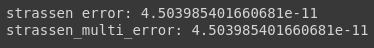
\includegraphics[width=0.8\textwidth]{images/res1.png}
\caption{Сравнение погрешностей}
\label{fig:img1}
\end{figure}

Графики зависимости времени выполнения от размерности матриц приведены на рисунке ~\ref{fig:img2}.

\begin{figure}[H]
\centering
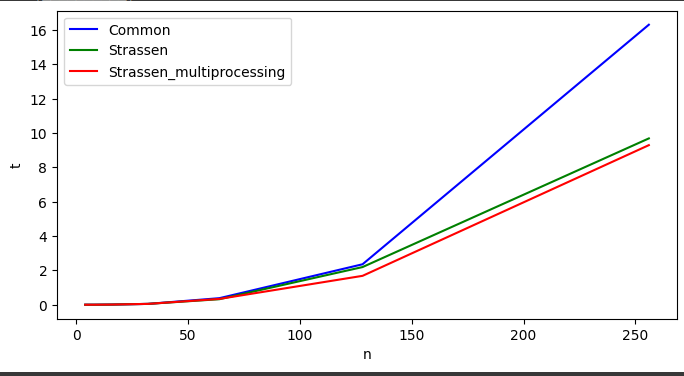
\includegraphics[width=0.8\textwidth]{images/res2.png}
\caption{Графики зависимости t от N}
\label{fig:img2}
\end{figure}


\section{Выводы}
В рамках данной лабораторной работы был реализован метод Штрассена, а также его многопоточная модификация. Также было проведено сравнение времени выполнения этих методов и обычного метода перемножения матриц в зависимости от размерности матрицы. Было установлено, что с ростом размерности метод Штрассена и его модификация демонстрируют куда лучший результат, нежели стандартный метод.
\end{document}